\section{Estado del Arte}

En este apartado se expone una investigación las plataformas de crowdfunding actuales donde se destaca que métodos se aplican para evitar proyectos fraudulentos, y plantear una solución para mejorar el sistema actual que usan dichas plataformas.

\bigskip

También se explica en detalle que es una Blockchain y como funciona, además entrar en profundidad en el funcionamiento del Protocolo Ethereum y otras tecnologías que se usarán para desarrollar el trabajo.

\subsection{Plataformas de Financiación Actuales}

A continuación se describe un ejemplo representativo de las plataformas de crowdfunding y gestión de fondos, tanto en web2\footnote{Terminología que referencia la arquitectura tecnológica web centralizada, más común conocida como arquitectura cliente - servidor.} como en web3\footnote{Terminología que referencia la arquitectura tecnológica web descentralizada, también conocidas como dapps: aplicaciones descentralizadas desplegadas en una blockchain.}.

\subsubsection{Kickstarter}

Kickstarter\cite{ContributorstoWikimediaprojects2023Jan} es una corporación de beneficio público estadounidense con sede en Brooklyn, Nueva York, que mantiene una plataforma global de financiación colectiva centrada en la creatividad. La misión declarada de la empresa es \quotes{ayudar a dar vida a proyectos creativos}.

\bigskip

Kickstarter lleva desde el 2013 recaudando fondos para proyectos de todo tipo, y por ello una de las plataformas que más experiencia tienen a la hora de enfrentarse a fraudes y vulnerabilidades similares.

\bigskip

La plataforma de Kickstarter funciona de la siguiente forma, cuando un proyecto se publica, kickstarter verifica la identidad del proponente del proyecto, además del fondo mínimo definido y los hitos propuestos para el proyectos. Una vez alcanzado el fondo mínimo definido, todos los fondos se traspasan al proponente, teniendo este total control sobre los fondos, y lo mismo ocurre para los hitos.

\bigskip

En este sistema, se deposita confianza en el recaudador, lo cual representa una debilidad, ya que si el proyecto resulta fraudulento o no se completa el recaudador es responsable de reembolsar lo recaudado a los inversores, aunque no exista una obligación legal. Para crear conciencia e informar a los inversores al respecto, Kickstarter publicó un artículo\cite{BibEntry2023Jan} detallando el proceso de validación y verificación de los proyectos permitidos en su plataforma web. Sin embargo, se insinúa que la responsabilidad final de los fondos recae en el inversor y en su juicio personal sobre el proyecto en el que decida invertir.

\bigskip

Este articulo, y además el ToS de la plataforma confirma que la única forma de recibir un reembolso después de que un proyecto haya recaudado el mínimo acordado es mediante una solicitud formal al propio proponente.

\bigskip

Kickstarter no se hace responsable de los fondos recaudados en caso de que el proyecto no pueda desarrollarse, o si algún hito no se pueda llegar a alcanzar. Esto incluye situaciones como por ejemplo que el proponente deje de comunicarse con sus inversores a través de la plataforma entre otros.

\bigskip

Esto permite que agentes maliciosos puedan proponer proyectos que mediante una campaña publicitaria logre convencer a los inversores de que el proyecto en el que están invirtiendo es factible, y al recaudar la cantidad acordada ignorar el desarrollo del proyecto y quedarse con lo recaudado.

\bigskip

Esto es un hecho ya que KickStarter tiene un amplio historial de proyectos fraudulentos, estafas, proyectos inviables, los cuales al final ninguno de los inversores recibieron el reembolso.\cite{kscam1}\cite{kscam2}\cite{kscam3}\cite{kscam4}\cite{kscam5}

\bigskip

Podemos asegurar que toda plataforma de recaudación de fondos que siga los mismo principios que esta tendrá las mismas flaquezas y se verá afectada de forma similar con respecto a la aparición de proyectos fraudulentos.

\subsubsection{Indiegogo}

Indiegogo es un sitio web estadounidense de crowdfunding fundado en 2008 por Danae Ringelmann, Slava Rubin y Eric Schell. Su sede se encuentra en San Francisco, California. El sitio es uno de los primeros sitios en ofrecer financiación colectiva. Indiegogo permite a las personas solicitar fondos para una idea, una organización benéfica o una empresa nueva. \cite{ContributorstoWikimediaprojects2022Aug}

\bigskip

Indiegogo, al igual que Kickstarter, es una plataforma web2 de financiamiento colectivo  en línea que permite a los emprendedores, creadores y organizaciones recaudar fondos para sus proyectos, productos o ideasm, y la cual también posee un FAQ\cite{indiegogohelp} describiendo en detalle los pasos los cuales debería seguir un inversor si el proyecto en el que ha invertido no logra desarollarse.

\bigskip

En este documento se confirma la misma situación que en la plataforma Kickstarter. El curso de acciones a realizar es par con el inversor y el proponente únicamente, la plataforma no se responsabiliza de los fondos ni realiza un seguimiento de los hitos del proyecto. 

\bigskip

La fiabilidad del proyecto recae sobre los comentarios y opiniones propuestas por anteriores inversores, por ello todo el proceso de reputación del proyecto recae sobre la comunidad.

\subsubsection{Crowdfunder}

Crowdfunder es una plataforma web2 de recaudación de fondos orientada a caridades, comunidades, empresas y individuales. Localizada en UK, esta plataforma tiene reputación por ser una de las plataformas más usadas sin ámbito de desarrollo de proyectos, donde sus fondos se usan para financiar todo tipo eventos y trabajos.

\bigskip

Esta plataforma usa un sistema idéntico al de IndieGogo y Kickstarter, incluido el relevo de la responsabilidad de la veracidad de los proyectos a la propia comunidad \cite{crowdfunderhelp}. La plataforma no se hace cargo de las perdidas ocasionadas en caso de haber financiado un proyecto fraudulento, y recae en la comunidad reportar y revisar este tipo de proyectos.

\newpage

\subsubsection{GitCoin}

Gitcoin\cite{qayum2020self} es una plataforma web3 que utiliza la tecnología blockchain para conectar a desarrolladores y creadores de contenido con oportunidades de financiamiento y trabajo en proyectos de código abierto. Esta plataforma se enfoca en fomentar la colaboración y el desarrollo sostenible de la comunidad de código abierto.

\bigskip

A través de esta plataforma, los desarrolladores pueden encontrar oportunidades de trabajo y financiamiento para sus proyectos de código abierto, mientras que los creadores de contenido pueden ganar dinero por la producción de tutoriales y documentación de proyectos. La plataforma utiliza un token llamado GTC (Gitcoin Coin) como medio de pago para las contribuciones de la comunidad.

\bigskip

Esta también ofrece herramientas y recursos para la gestión de proyectos de código abierto, incluyendo un tablero de tareas y un sistema de seguimiento de problemas. Esto ayuda a mantener la transparencia y la responsabilidad en el desarrollo de proyectos de código abierto y fomenta una cultura de colaboración y aprendizaje continuo.

\bigskip

Aunque Gitcoin proporciona un espacio para financiar y colaborar en proyectos de código abierto, la adopción y el conocimiento de la plataforma aún pueden ser limitados en comparación con otras soluciones de financiamiento. Además, la naturaleza descentralizada de las criptomonedas y la falta de regulación pueden generar cierto grado de incertidumbre y volatilidad en las recompensas recibidas por los desarrolladores.

\bigskip

El sistema sobre el que se ejecuta la plataforma utiliza el protocolo blockchain Ethereum para gestionar sus activos y contratos inteligentes. La plataforma se basa en la tecnología de blockchain para crear un sistema seguro, transparente y descentralizado para la gestión de fondos y la distribución de recompensas.

\bigskip

Los contratos inteligentes de Gitcoin están desplegados en la red principal de Ethereum (también conocida como Ethereum Mainnet). Esto significa que todas las transacciones y operaciones que se realizan en la plataforma se registran en la cadena de bloques de Ethereum, esto garantiza la inmutabilidad y la transparencia de los datos.


\newpage

\subsubsection{CoinStarter}

CoinStarter\cite{singh2021introduction}, fundada en 2017 por Cornell Holloway, es una de las plataformas web3 de financiamiento colectivo más grandes basadas en criptomonedas. La estructura de esta plataforma, impulsada por la comunidad, ofrece una excelente manera de conectar a los donantes con los proyectos en los que creen de forma más intrínseca.

\bigskip

Para comenzar a invertir en CoinStarter se requiere una membresía. Esta membresía permite a las causas generar sus propios modelos de suscripción para obtener ingresos. Esto implica que los usuarios pagan una tarifa mensual para acceder a la extensa comunidad de la plataforma. No obstante, las donaciones también están sujetas a tarifas de transacción.

\bigskip

Uno de los aspectos destacados de CoinStarter es su diseño simplificado que permite a los usuarios, incluso aquellos que no tienen experiencia en criptomonedas, crear sus propias campañas de financiamiento colectivo. La plataforma es flexible y cuenta con salas de chat estilo Discord, que facilitan a los proyectos la identificación de audiencias objetivo y la comprensión de sus necesidades.

\bigskip

Los contratos inteligentes de CoinStarter están desplegados en la red Ethereum.
Los beneficios de utilizar CoinStarter incluyen la posibilidad de acceder a una amplia comunidad de inversores y donantes interesados en proyectos basados en criptomonedas, la facilidad de uso para usuarios con poca experiencia en criptomonedas y la seguridad y confianza proporcionadas por la red Ethereum y sus contratos inteligentes. Además, la plataforma fomenta una mayor conexión entre donantes y proyectos, permitiendo a los creadores adaptar sus campañas a las necesidades de su público objetivo.

\bigskip

Los negativo por otro lado es el propio requerimiento de una membresia que incluye una tarifa mensual, lo que podría disuadir a algunos usuarios. Además, las donaciones están sujetas a tarifas de transacción, lo que podría reducir la cantidad de fondos que llegan a los proyectos.

\newpage

\subsubsection{Tecra Space}

Al igual que CoinStarter, Tecra Space es una plataforma web3 de financiamiento colectivo que adopta un enfoque más tradicional. Este espacio descentralizado permite la inclusión de proyectos diversos que involucran patentes, activos digitales y otros derechos de propiedad intelectual, los cuales se desglosan y tokenizan.

\bigskip

La plataforma facilita a los desarrolladores la inclusión de sus proyectos y la oferta de plazos variados para los tokens y sus recompras. Además, Tecra Space permite que los proyectos se incluyan con diferentes niveles de inversión y ventajas para los inversores, como acceso a productos o servicios digitales, menciones, créditos, ilustraciones temáticas, entre otros.

\bigskip

Tecra Space incluye una amplia gama de proyectos, como videojuegos, aplicaciones descentralizadas, operaciones de minería y servicios de energía renovable. Los contratos inteligentes de Tecra Space están desplegados en la red Ethereum, garantizando seguridad y confiabilidad en las transacciones y procesos automatizados.

\bigskip

En cuanto a los beneficios de Tecra Space, se destacan la versatilidad en la inclusión de proyectos, la posibilidad de ofrecer ventajas personalizadas a los inversores y la descentralización a través de la tecnología blockchain. Esto permite una mayor flexibilidad y alcance para los creadores de proyectos y los inversores.

\bigskip

Por otro lado, los aspectos negativos incluyen la complejidad asociada a la tecnología blockchain y criptomonedas para usuarios sin experiencia en el área, y la incertidumbre regulatoria en torno a la tokenización de activos intangibles. Estos aspectos pueden representar desafíos tanto para los creadores de proyectos como para los inversores en la plataforma.

\newpage

Para detallar las características estas plataformas, a continuación se muestra una tabla comparativa entre las plataformas mencionadas previamente, basándose en el modelo de financiamiento (A), moneda utilizada (B), industria principal (C),  Comisión (D), plazo de financiamiento (E), distribución (F).

\begin{table}[ht]
\centering
\begin{tabular}{@{}lllllll@{}}
\hline
    & \textbf{Kickstarter} & \textbf{Indiegogo} & \textbf{Crowdfunder} & \textbf{GitCoin} & \textbf{CoinStarter} & \textbf{Tecra Space} \\ \hline
    A & All-or-nothing & Equidad & Flexible & Recompensas & ICO / STO & ICO / STO \\
    B & Fiat & Fiat / Crypto & Fiat & Crypto & Crypto & Crypto \\
    C & Tecnología & Tecnología & StarUps & Software & Blockchain & Ciencia \\
    D & 5\% & 5\% & Varía & 0\% & Varía & Varía \\
    E & Hasta 60 días & Flexible & Flexible & Flexible & Flexible & Flexible \\
    F & Centralizado & Centralizado & Centralizado & Varía & Descentralizado & Descentralizado \\
\hline
\end{tabular}
\caption{Estado del Arte - Tabla comparativa de plataformas de crowdfunding}
\label{tab:comparativa}
\end{table}


\newpage

\subsection{Conclusiones respecto al estado del arte}

De esta investigación se puede sacar en claro que las plataformas de crowdfunding actuales desplegadas que no son descentralizadas relevan su responsabilidad con el inversor, ya que en caso de tomar dicha responsabilidad la propia plataforma debería emprender acciones legales en contra del proponente en los casos de haber ejecutado una estafa o fraude.\cite{1}

\bigskip

También podemos ver que la mayoría de las plataformas están reguladas por la comunidad, aunque la decisión final esté en manos de un administrador que posee la capacidad de alterar cualquier dato.

\bigskip

El mismo administrador en un futuro podría suponer una flaqueza para el sistema, ya que dependiendo de como esté desarrollado el sistema, este puede poseer la autoridad de enmascarar cualquier estafa publicada en la plataforma.

\bigskip

Para que nuestro sistema no sufra dichas flaquezas necesitamos que los activos recaudados puedan ser congelables\footnote{Actividad que paraliza la transferencia de fondos.} y que la plataforma esté totalmente controlada por la comunidad de una forma balanceada.

\bigskip

Además, una blockchain descentralizada, esta al ser inmutable no posee los riesgos externos comparados con el uso de un sistema centralizado, como por ejemplo que el recaudador o un administrador malicioso pueda modificar o eliminar una propuesta de proyecto sin dejar rastro de este.

\bigskip

También, a través de los Smart Contracts, se puede crear un sistema de gobernanza que no necesite ningún administrador, y que esté totalmente regulado por la comunidad.

\bigskip

Para este trabajo es importante que la blockchain sea de acceso publico, debido a que queremos que la comunidad tenga el control sobre los activos, y cualquier inversor pueda trazar los activos que se han invertido en un proyecto. Además, la red debe ser modular, para evitar los problemas de escalado que tienen las redes blockchain monolíticas a largo plazo.

\bigskip

El consenso de la red blockchain debe ser Proof of Stake, ya que es la forma más cómoda para que los usuarios puedan participar en la red, sin que haya discriminación de recursos.

\bigskip

La discriminación de recursos en las redes blockchains se da cuando estas usan el consenso POW. Este consenso da pié a  que un nodo minero pueda verificar transacciones más rápido que el resto de nodos, así obteniendo un beneficio mayor y todo debido a que los recursos computacionales del nodo son mayores. Esto afecta a la red, ya que a largo plazo provoca que el resto de nodos con menos recursos obtengan un beneficio cada vez menor. 

\bigskip

En el siguiente capitulo se describe más en detalle la tecnología y la configuración a usar óptima para la propuesta de solución.

\newpage

\section{Contexto Tecnológico}

En este apartado se describe y explica en profundidad las tecnologías blockchain, como funcionan y que beneficios y contras nos provee.

\subsection{Las redes Blockchain}

Una blockchain\cite{di2017blockchain} no es más que una red de ordenadores que funcionan de forma descentralizada, esto significa que los ordenadores no dependen del resto de los ordenadores de la red para seguir con el correcto funcionamiento, pero dicha descentralización fortalece el objetivo de la red.

\bigskip

Aunque hayan diferentes tipos de blockchain orientadas a diferentes objetivos, todas tienen una función común, y es la de ejercer como una base de datos. Mediante la criptografía, la propia red blockchain se fortalece con la descentralización, proveyendo de trazabilidad, inmutabilidad y privacidad.

\bigskip

Los datos guardados se replican en la red, y se almacenan de forma consecutiva y secuencial en cada nodo. Al almacenar un nuevo dato se crea una transacción en la blockchain firmada por el usuario que añade dicho dato, así ejerciendo como un libro mayor descentralizado en el cual se guarda que transacción ha emitido cada usuario.

\bigskip

Esta transacción es un mero registro con varios datos: un identificativo del usuario que ha insertado el dato, la firma del usuario asociado al dato a insertar y un hash\footnote{Algoritmo matemático que transforma el conjunto de datos de entrada en una expresión alfanumérica que tiene una longitud predeterminada.} de la combinación del dato insertado anteriormente y el dato actual así formando una Merkle Tree\cite{merkeltree}. Y una vez que se han insertado varios datos, estos se agrupan en un bloque y se archivan para facilitar su acceso.


\begin{figure}[H]
        \centering
        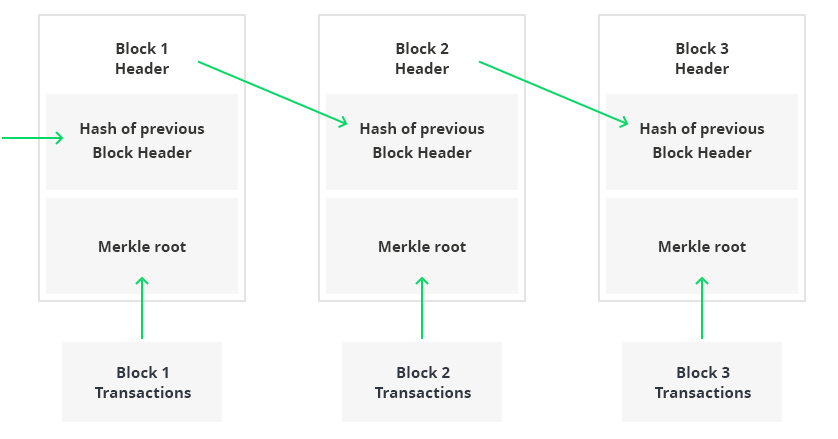
\includegraphics[width=1\textwidth]{img/capturas/blockchain.png}
        \caption{Estructura de una Blockchain.}
        \label{fig:configApi}
\end{figure}


De esta forma, se genera una arquitectura basada en bloques de datos que enlaza ( mediante el hash ) cada transacción sucesivamente ( BlockChain ).

\bigskip

Como se ha mencionado, cada transacción posee un hash que representa la integridad de todos los datos anteriores. Mediante el hash de la ultima transacción de esta cadena, se puede validar que ningún dato ha sido alterado.


\subsubsection{Inmutabilidad y Trazabilidad}

La inmutabilidad se logra a través de un proceso llamado \quotes{consenso} usando el hash de cada dato. En este proceso, un grupo de nodos verifica y valida cada transacción antes de agregarla a la blockchain. Una vez que se agrega un bloque, no puede ser modificado o eliminado.

\begin{figure}[H]
        \centering
        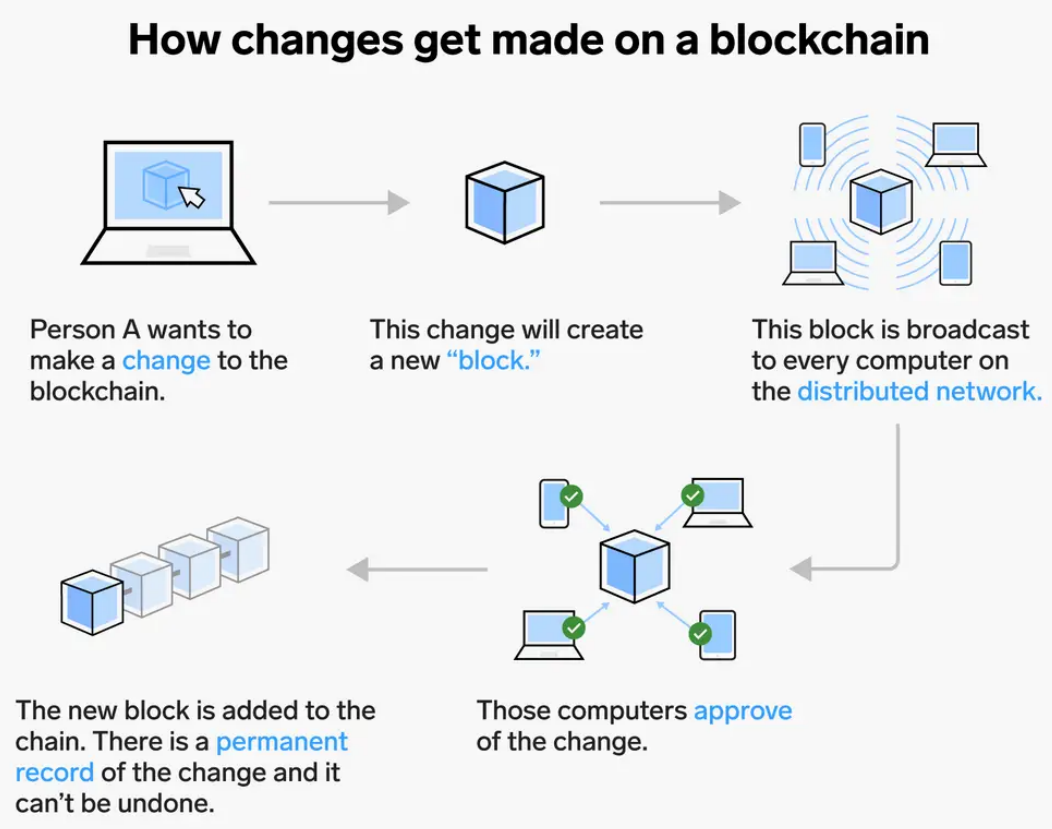
\includegraphics[width=0.9\textwidth]{img/capturas/cambios.png}
        \caption{Funcionamiento de una Blockchain - Business Insider.}
        \label{fig:configApi}
\end{figure}


\bigskip

La trazabilidad se logra porque cada transacción en la blockchain está vinculada al usuario que la ha emitido, lo que permite seguir la pista de quién hizo qué y cuándo.

\bigskip

Mientras más nodos posea una red, más difícil será atacarla, ya que cada nodo de la red posee una copia exacta de los datos, de esta forma se valida la integridad de los datos entre los nodos de la red.

\subsubsection{Consenso y tipos de consensos}

El consenso\cite{consensus} en una blockchain es el proceso por el cual los nodos de la red acuerdan sobre la veracidad de las transacciones y la creación de nuevos bloques en la cadena. Es esencial para garantizar la integridad y seguridad de la red y evitar varias formas de fraude.

\bigskip

Existen varios tipos de consenso en las blockchains, algunos de los más comunes incluyen:

\paragraph{Proof-of-Work (PoW)} El consenso PoW es un sistema en el que los nodos mineros compiten para resolver un problema matemático complejo y crear un nuevo bloque. El primer nodo que lo resuelve recibe una recompensa en criptoactivos ( critomonedas / tokens ).

\bigskip

Pros:
\begin{itemize}

    \item Seguridad: El sistema Proof of Work proporciona una forma robusta de proteger una red blockchain contra ataques y manipulaciones.

    \item Decentralización: Al requerir que los mineros compitan entre sí para validar bloques, la red no está controlada por una sola entidad, sino por un grupo descentralizado de participantes.

    \item Immutabilidad: Una vez que un bloque es validado y agregado a la cadena, no se puede modificar sin la necesidad de recrear toda la cadena desde el bloque cambiado, lo que resulta en una inalterabilidad más alta.
    
\end{itemize}

Cons:
\begin{itemize}

    \item Consumo de energía: El proceso de minería en sí consume una gran cantidad de energía, lo que resulta en un impacto ambiental negativo.

    \item Lentitud: El tiempo requerido para validar un bloque puede ser demasiado largo, lo que resulta en una menor escalabilidad y eficiencia.

    \item Centralización: A medida que los costos de minería aumentan, solo las grandes corporaciones con acceso a grandes cantidades de hardware y energía pueden competir en la minería, lo que puede resultar en una centralización y una menor descentralización de la red.

\end{itemize}

\paragraph{Proof-of-Stake (PoS)} El consenso PoS es un sistema en el que los nodos validadores son seleccionados aleatoriamente para validar las transacciones y insertar nuevos bloques basados en la cantidad de criptoactivos que poseen y están dispuestos a \quotes{apostar}.

\bigskip

Pros:

\begin{itemize}
    \item Reducción de la energía: El sistema Proof of Stake consume significativamente menos energía que Proof of Work, lo que resulta en un impacto ambiental significativamente menor.
    \item Mayor escalabilidad: Al requerir menos recursos para validar bloques, la red es más eficiente y escalable.
    \item Descentralización mejorada: Al permitir que los validadores seleccionados sean elegidos por la cantidad de criptomonedas que poseen, el sistema Proof of Stake puede resultar en una mayor descentralización y una menor centralización en comparación con Proof of Work.
\end{itemize}

Cons:

\begin{itemize}
    \item Vulnerabilidad a ataques: Si un validador malintencionado tiene una participación significativa en la red, puede controlar la validación de los bloques y llevar a cabo ataques.
    \item Falta de inmunidad ante manipulaciones: Al no requerir un esfuerzo computacional para validar bloques, el sistema Proof of Stake es más vulnerable a manipulaciones y ataques.
    \item Dificultad para participar: Al requerir que los validadores posean una cantidad significativa de criptomonedas, el sistema Proof of Stake puede resultar en una barrera para la participación de nuevos usuarios en la red.
\end{itemize}

\paragraph{Delegated Proof-of-Stake (DPoS)} El consenso DPoS es un sistema en el que los nodos validadores son elegidos por la comunidad de usuarios a través de un sistema de votación.

\bigskip

\begin{itemize}
    \item Mayor escalabilidad: Al limitar el número de validadores en la red, el sistema Delegated Proof of Stake permite una mayor velocidad de procesamiento y una mejor escalabilidad en comparación con otros sistemas de consenso.
    \item Reducción de costos: Al requerir menos recursos para validar bloques, DPoS resulta en una reducción de los costos de hardware y electricidad en comparación con otros sistemas de consenso.
    \item Descentralización mejorada: Al permitir a los usuarios elegir a los validadores, DPoS puede resultar en una descentralización más efectiva y una menor centralización en comparación con sistemas de consenso centralizados.
\end{itemize}

Cons:

\begin{itemize}
    \item Vulnerabilidad a la manipulación: Al permitir a los usuarios elegir a los validadores, DPoS es más vulnerable a la manipulación y a la influencia de grupos con intereses específicos.
    \item Centralización potencial: Si un pequeño grupo de validadores controla una gran cantidad de la red, puede resultar en una centralización y una falta de descentralización.
    \item Falta de inmunidad ante ataques: Al tener un pequeño número de validadores, la red puede ser más vulnerable a ataques y manipulaciones en comparación con otros sistemas de consenso.
\end{itemize}

\newpage

\paragraph{Practical Byzantine Fault Tolerance (PBFT)} El consenso PBFT es un algoritmo en el que los nodos validadores se comunican entre sí para acordar la veracidad de las transacciones y la creación de nuevos bloques.

\bigskip

Pros:

\begin{itemize}
    \item Alta disponibilidad: El algoritmo Practical Byzantine Fault Tolerance (PBFT) se diseñó específicamente para manejar la falla de nodos y garantizar la disponibilidad de la red incluso en presencia de fallas.
    \item Velocidad y escalabilidad: PBFT permite una velocidad de procesamiento rápida y una mejor escalabilidad en comparación con otros sistemas de consenso basados en pruebas.
    \item Seguridad mejorada: Al requerir un consenso entre los nodos en la red antes de validar un bloque, PBFT mejora la seguridad y reduce la vulnerabilidad a ataques en comparación con otros sistemas de consenso.
\end{itemize}

Cons:

\begin{itemize}
    \item Centralización potencial: Al requerir un consenso entre los nodos en la red, PBFT puede resultar en una centralización si un pequeño número de nodos controla una gran cantidad de la red.
    \item Dificultad para implementar: El algoritmo PBFT es más complejo que otros sistemas de consenso y puede ser más difícil de implementar y mantener.
    \item Requerimiento de recursos: PBFT requiere una cantidad significativa de recursos para funcionar de manera efectiva, lo que puede resultar en una barrera para la participación de nuevos usuarios en la red.
\end{itemize}

\bigskip

Cada tipo de consenso tiene sus propios pros y contras en términos de seguridad, escalabilidad, eficiencia y costo, y la elección de un sistema de consenso puede afectar significativamente el funcionamiento y desempeño de una blockchain.

\newpage

\subsubsection{Nodos y tipos de Nodos}

Los nodos\cite{nodes} son los ordenadores que forman parte de la red blockchain, cada nodo puede tener una responsabilidad, y dependiendo del tipo de blockchain y para lo que esté orientada, este tipo de nodos pueden ser diferentes. Basada en esta responsabilidad los nodos más comúnes son los siguiente:

    \paragraph{Nodo Validador}
    
    Un nodo validador o nodo minero en una blockchain es un participante especial que se encarga de realizar la función de consenso y crear nuevos bloques en la cadena. 
    
    \bigskip
    
    Los nodos validadores o mineros verifican las transacciones y las incluyen en un nuevo bloque siguiendo un protocolo de consenso específico, como Proof-of-Work (PoW) o Proof-of-Stake (PoS). 
    
    \bigskip
    
    Al crear nuevos bloques y agregarlos a la cadena, estos nodos ayudan a mantener la integridad y seguridad de la red y son recompensados con criptomonedas o tokens.
    
    \paragraph{Nodo Completo}
    
    Un nodo completo en una blockchain es un participante que mantiene una copia completa de la blockchain y verifica todas las transacciones y bloques antes de aceptarlos y agregarlos a la cadena.
    
    \bigskip
    
    Estos nodos cumplen un papel importante en mantener la integridad y seguridad de la red, ya que verifican que todas las transacciones cumplan con las reglas y protocolos establecidos de la red.
    
    \paragraph{Nodo Parcial}
    
    Un nodo parcial en una blockchain es un participante que mantiene solo una parte de la información de la blockchain, en comparación con un nodo completo que mantiene una copia completa de la cadena.
    
    \bigskip
    
    Estos nodos pueden ser menos seguros y confiables que los nodos completos, ya que dependen de la información proporcionada por otros nodos para validar las transacciones y agregar bloques a la cadena.
    
    \bigskip
    
    Sin embargo, también pueden ser más eficientes en términos de recursos y pueden cumplir un papel útil en la escalabilidad de la red.
    
    \paragraph{Nodo Archivo}
    
    Un nodo archivo en una blockchain es un nodo que mantiene una copia completa de la historia de todas las transacciones y bloques en la cadena. Este tipo de nodo está diseñado para proporcionar acceso a información histórica y auditable de la red a los usuarios y aplicaciones que la utilizan.
    
    \bigskip
    
    Los nodos archivo son diferentes a los nodos completos, ya que los nodos completos están activamente involucrados en la verificación y el procesamiento de transacciones, mientras que los nodos archivo están diseñados principalmente para proporcionar acceso a la información histórica de la blockchain.
    
    \bigskip
    
    Estos nodos son útiles para aplicaciones que requieren acceder a información detallada sobre transacciones y eventos pasados en la blockchain, como auditorías financieras, análisis de datos y supervisión reguladora. Sin embargo, debido a la gran cantidad de datos que deben almacenar, los nodos archivo pueden requerir una gran cantidad de recursos de hardware y ancho de banda.
    
    \paragraph{Nodo de Autoridad}
    
    Un nodo de autoridad en una blockchain es un nodo especial que se confía explícitamente para proporcionar información veraz y actualizada sobre la blockchain. Estos nodos suelen ser administrados por organizaciones confiables, como bancos, gobiernos u organizaciones reguladoras, y están diseñados para proporcionar información sobre la blockchain a terceros que necesitan verificar transacciones o eventos en la red.
    
    \bigskip
    
    Este tipo de nodos se usan en entornos regulados o en los que se requiere una mayor transparencia y confianza en la información de la blockchain, como en el caso de aplicaciones financieras o de seguimiento de suministro. Sin embargo, también pueden ser criticados por ser un punto centralizado de falla y por socavar la descentralización y la confianza en la red.

\subsubsection{Cuentas y Carteras}

Para que un usuario pueda interactuar con una blockchain, este deberá usar una cuenta. Las cuentas en una blockchain están formadas por 2 claves, una publica y otra privada, la clave publica se usa para identificar la cuenta, y la privada se usa para acceder y firmar las transacciones.

\bigskip

Las cuentas sirven para tener un registro público de transacciones y saldo. Para interactuar con una cuenta se requiere una \quotes{cartera}, que es el nombre que se le da a un software que permite a un usuario controlar sus cuentas y realizar transacciones. La cartera puede ser un software en línea o un dispositivo físico que almacena las claves privadas asociadas con las cuentas del usuario en la blockchain.

\bigskip

\newpage

\subsubsection{Accesos y tipos de acceso}
Dependiendo del objetivo y tipo de blockchain ( empresarial, gubernamental, publica, etc ), el acceso a está puede clasificarse en 4 tipos generales.

\begin{figure}[H]
        \centering
        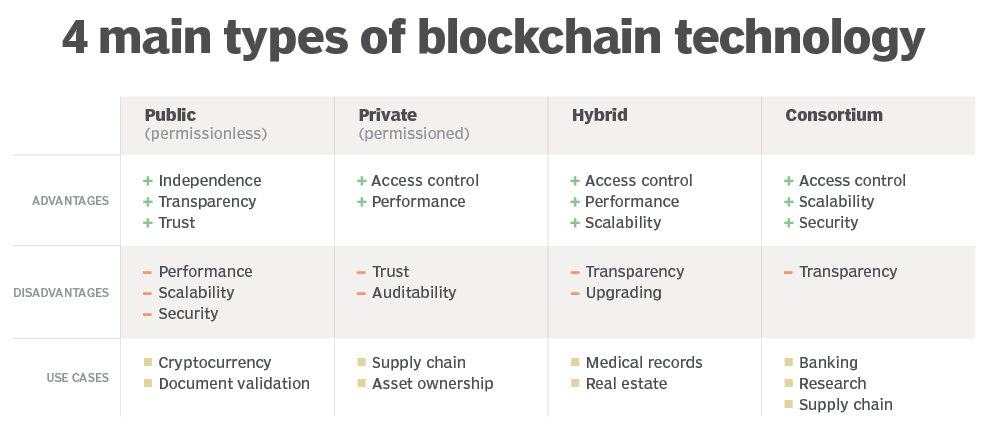
\includegraphics[width=1\textwidth]{img/capturas/types.png}
        \caption{Ventajas y desventajas de los tipos de blockchain basado en su acceso - Tech Target Media.}
        \label{fig:configApi}
\end{figure}

    \paragraph{Publica}
    Una blockchain pública es una blockchain abierta y accesible para cualquier persona. Todos pueden leer, escribir y participar en la red. Ejemplos incluyen Bitcoin y Ethereum.
    
    \paragraph{Privada}
    Una blockchain privada es una blockchain que restringe el acceso a un grupo específico de participantes. Este tipo de blockchain se utiliza en aplicaciones empresariales y puede ser administrados por una organización o un grupo de organizaciones.
    
    \paragraph{Híbrida}
    Una blockchain híbrida es una combinación de una blockchain pública y privada. En una blockchain híbrida, un grupo de nodos es responsable de validar las transacciones y mantener la integridad de la red, mientras que otros nodos tienen acceso de lectura.
    
    \paragraph{Consorcio}
    Una blockchain de consorcio es similar a una blockchain federada, pero está controlado por un grupo de organizaciones que trabajan juntas. Este tipo de blockchain se utiliza en aplicaciones empresariales y permite un mayor control y privacidad de las transacciones de la red.

\newpage

\subsubsection{Blockchains monolíticas y modulares}

También, dependiendo del tipo de arquitectura existen 2 clasificaciones de blockchains: Monolítico y Modular.

\begin{figure}[H]
        \centering
        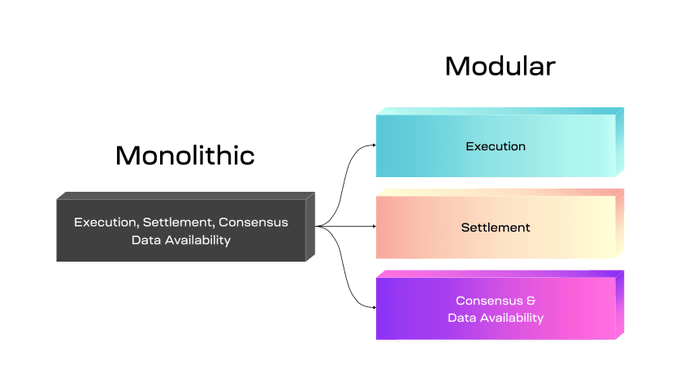
\includegraphics[width=0.7\textwidth]{img/capturas/monovsmodu.png}
        \caption{Diagrama representativo de las blockchains monolíticas y modules - Médium.}
        \label{fig:configApi}
\end{figure}

La diferencia entre monolíticas y modulares es la forma en que están diseñados y organizados los componentes. Las blockchains monolíticas tienen todas las funciones en un solo módulo, mientras que las blockchains modulares tienen diferentes funciones en módulos separados.

\bigskip

Las blockchains modulares son las más usadas hoy en día, porque permiten relevar la carga de trabajo de un módulo a otras blockchains. A esta práctica se le conoce como Layer 2\cite{BinanceAcademy2023Feb}, que describe un set especifico de soluciones de escalado para la blockchain.

\begin{figure}[H]
        \centering
        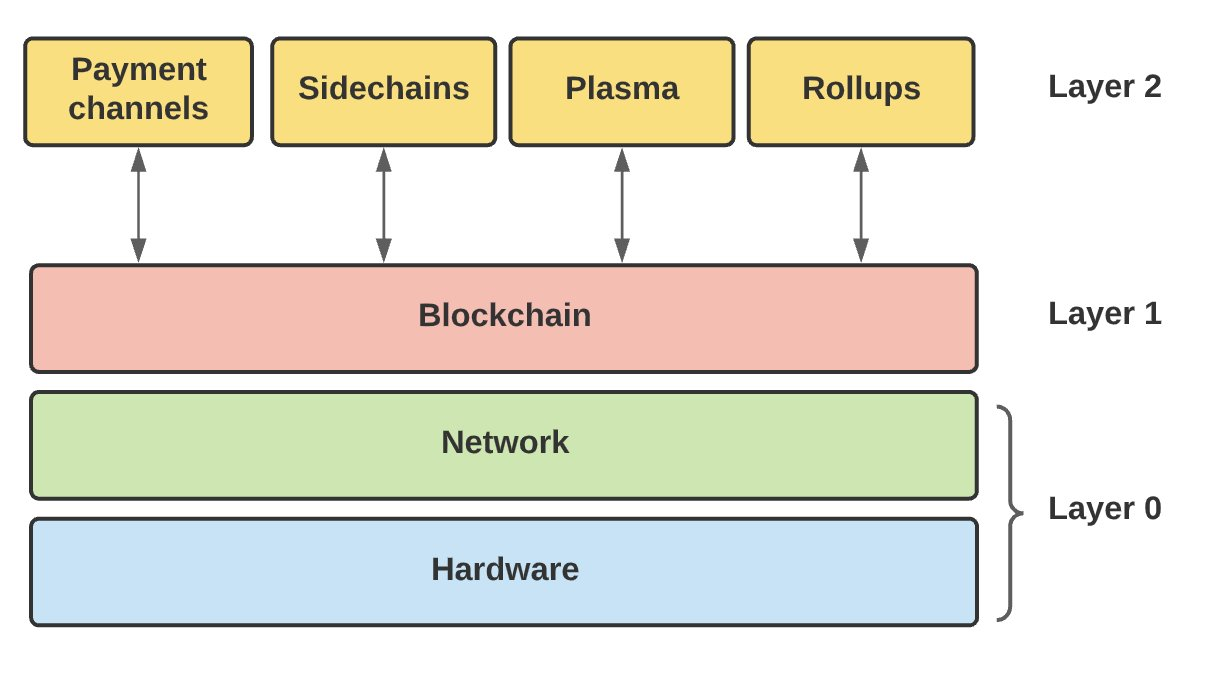
\includegraphics[width=0.7\textwidth]{img/capturas/layer2.jpg}
        \caption{Representación de las layers del 0 al 2 de una blockchain.}
        \label{fig:configApi}
\end{figure}

\paragraph{Criptomonedas}

Las criptomonedas, aunque no sean totalmente necesarias en una blockchain, sigue siendo una parte fundamental para muchos ecosistemas en los cuales se requiere de un incentivo para minar o validar transacciones.

\bigskip

Las criptomonedas surgieron originalmente del Bitcoin, una de las primeras redes blockchain. Esta red fue creada con el objetivo de crear el primer criptoactivo de Internet, una moneda la cual no se vería influenciada por empresas o gobiernos, y que fuese de libre uso para todas las personas.

\bigskip

Hoy en día existen blockchains orientadas a todo tipo de finalidades, pero la mayoría poseen una criptomoneda nativa a cada red. Esta criptomoneda se usa para recompensar y fomentar que las personas usen la red. Por ejemplo, la propia red recompensa a los mineros y validadores al prestar su capacidad de computo para verificar las transacciones de la red.

\subsubsection{Smart Contracts - Chain Code}

Algunas blockchains como Ethereum permiten aprovechar la capacidad computacional de los nodos de la red, de tal forma la blockchain además de solo almacenar datos también puede ejecutar programas en los nodos.

\bigskip

Los Smart Contracts o también conocido como Chain-Code son programas que se ejecutan en la blockchain y permiten automatizar el cumplimiento de acuerdos digitales. Estos programas una vez desplegados son inmutables, por lo tanto las funciones y lógica definidas son inalterables.

\bigskip

Estos contratos pueden almacenar y transferir valores, activos o información en una forma segura, transparente y sin intermediarios, gracias a la inmutabilidad y descentralización de la blockchain.

\bigskip

De esta manera, los smart contracts permiten crear una red de confianza entre sus participantes sin la necesidad de terceros confiables.

\begin{figure}[H]
        \centering
        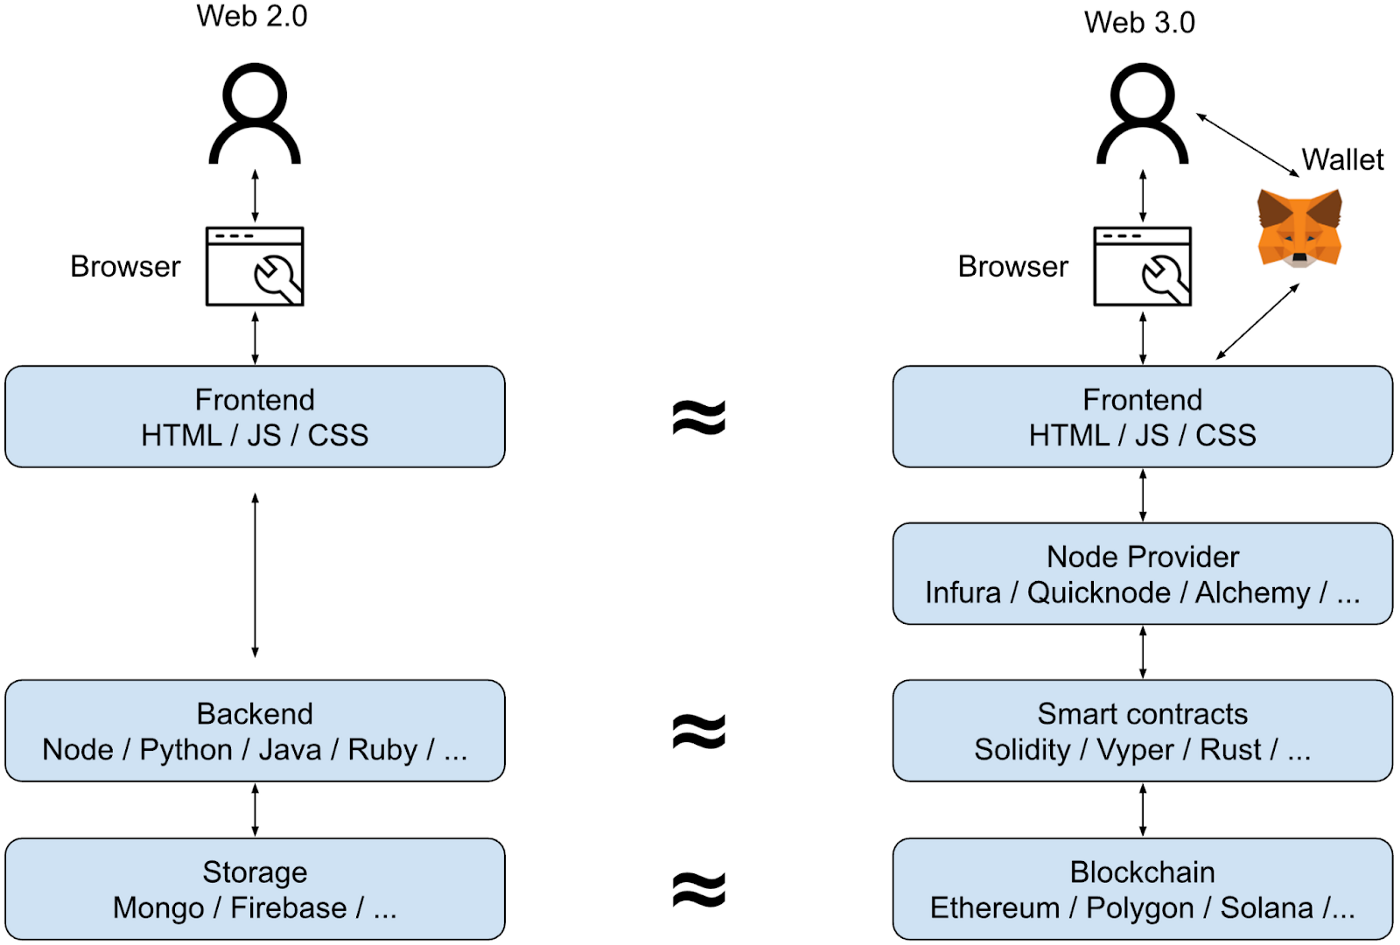
\includegraphics[width=0.7\textwidth]{img/capturas/web2vsweb3.png}
        \caption{Comparación entre web2 y web3 del proceso de interacción con aplicaciones.}
        \label{fig:configApi}
\end{figure}

\newpage

\subsection{Ethereum}

Ethereum\cite{Ethereum} es una blockchain publica modular, que soporta diferentes consensos, y basada en DLT con su propia criptomoneda y con la capacidad de almacenar datos y ejecutar lógica en sus nodos.

\bigskip

Esta última característica es la que la diferencia de la mayoría de blockchains de hoy en día, además de la posibilidad de poder clonar el proyecto, y desplegar una versión propia de esta blockchain, ya que el protocolo Ethereum es un proyecto de código abierto.

\subsubsection{El protocolo Ethereum}

El protocolo Ethereum\cite{gitether} es un proyecto desarollado en C++, Python y Go, que permite desplegar una blockchain personalizable.

\bigskip

El protocolo despliega una red basa en una estructura de blockchain y utiliza que propia criptomoneda, Ether (ETH), para compensar a los nodos en la red por el trabajo que realizan al validar y ejecutar las transacciones y contratos en la red.

\bigskip

Además, este protocolo permite la creación de tokens\cite{token} personalizados, lo que lo hace popular para la creación de proyectos de finanzas descentralizadas (DeFi) y aplicaciones descentralizadas (dApps). En otras palabras, el protocolo Ethereum es la base tecnológica sobre la cual se ejecuta la blockchain Ethereum.

\bigskip

Esto también significa que la blockchain Ethereum no es la única que ejecuta el protocolo Ethereum, por ejemplo Polygon, Telos, Cardano, Avalanche, TRON son redes blockchain con ciertas diferencias a la blockchain Ethereum pero que siguen ejecutando el mismo protocolo.


\subsubsection{Ethereum Virtual Machine}

La Máquina Virtual Ethereum (EVM)\cite{evm} es el motor de Ethereum, se encarga de almacenar todos los datos y de ejecutar las operaciones de los contratos inteligentes.

\bigskip

Además es entorno de ejecución de los contratos inteligentes. La EVM permite que los contratos se ejecuten de manera uniforme y segura en todos los nodos en la red, independientemente del hardware y del software que utilicen.

\bigskip

Mientras Ethereum tiene su propia criptomoneda nativa (Ether) que sigue casi exactamente las mismas reglas intuitivas, también permite una función mucho más poderosa: los contratos inteligentes. Para esta función más compleja, se requiere una analogía más sofisticada. 

\newpage

En lugar de un ledger distribuido\cite{dlt}, Ethereum es una máquina de estado distribuido. El estado de Ethereum es una estructura de datos grande que no solo contiene todas las cuentas y saldos, sino también un estado de la máquina, que puede cambiar de bloque a bloque de acuerdo a un conjunto de reglas preestablecidos y que puede ejecutar cualquier código de máquina. 

\begin{figure}[H]
    \centering
    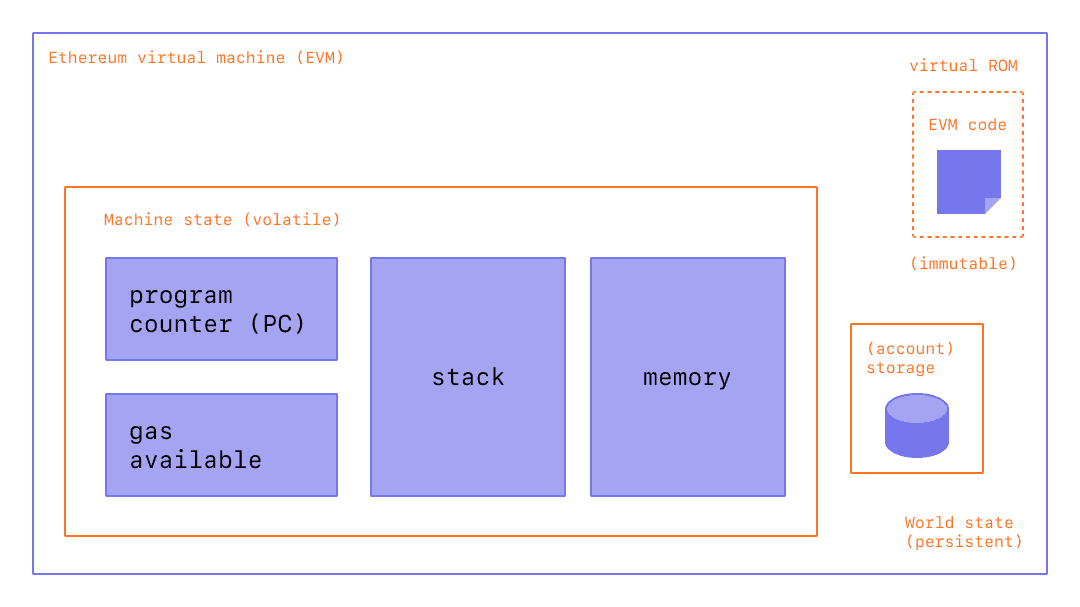
\includegraphics[width=1\textwidth]{img/capturas/EVM.png}
    \caption{Diagrama que representa la EVM - Ethereum.org .}
    \label{fig:configApi}
\end{figure}

Las reglas específicas para cambiar el estado de bloque a bloque están definidas por la EVM. Los contratos inteligentes se escriben en un lenguaje de programación de alto nivel, ya sea usando un lenguaje orientado a objetos mediante el uso de alguna librería como Viper\cite{Vyper} para Python, o mediante Solidity\cite{soliditylang}, y luego se compilan a instrucciones bytecode que se puede ejecutar en la EVM. Una vez que un contrato se ha implementado en la EVM, los usuarios pueden interactuar con él mediante transacciones en la red.

\bigskip

En resumen, la EVM es un entorno de ejecución seguro y uniforme para contratos inteligentes en la red Ethereum, que permite que los contratos se ejecuten de manera confiable y consistente en todos los nodos en la red.

\subsubsection{Funcionamiento de la EVM}

El EVM se comporta como lo haría una función matemática, dada una entrada, produce una salida determinista. Por lo tanto, es muy útil describir de manera más formal a Ethereum como si fuese una función de transición de estados.

\bigskip

En el contexto de Ethereum, el \quotes{state} es una enorme estructura de datos Merkle Patricia Trie modificada\cite{patricia}, que mantiene todas las cuentas vinculadas por hashes y se puede reducir a un solo hash raíz almacenado en la blockchain.

\subsubsection{Ejecución de la EVM}

La EVM se encarga de ejecutar instrucciones definidas ( OPCODES )\cite{opcodes}, que se ejecutan en la blockchain.

\bigskip


Para evitar que hayan bucles infinitos u otras instrucciones capaces de agotar los recursos de los nodos de la blockchain y para incentivar a los mineros a validar las transacciones que realiza una instrucción, cada instrucción tiene un coste en ETH definido en una unidad llamada GAS.

\subsubsection{Gas}

El gas es una unidad de medida del ETH, que se usa para medir cuánto ETH cuesta ejecutar una operación.\cite{gas} Esta medida se rige por la siguiente formula:

\bigskip

\centerline{gasUsado * precioGas = tarifaDelGas}

\bigskip

Dado que cada transacción requiere recursos computacionales para ejecutarse, cada transacción requiere una tarifa. Gas se refiere a la tarifa requerida para realizar una operación en Ethereum con éxito.

\bigskip

Debido a la variación de la carga de trabajo de los nodos de la blockchain, el precio del gas suele oscilar durante el día. Cada año, debido a que la red siempre está en continua expansión, el gas se vuelve ligeramente más caro.

\bigskip

Hay páginas como \textcolor{blue}{\href{https://etherscan.io}{\textbf{Etherscan}}}\footnote{\url{https://etherscan.io/}} que muestran el estado de la red, sus transacciones, y el precio estimado del gas durante el día.

\bigskip

El cálculo de la tarifa de las transacciones en gas funciona de la siguiente manera: 

\bigskip

\centerline{unidades de gas (límite) * (tarifa base + propina)}

\bigskip

Cuando un usuario ejecuta una instrucción, éste puede definir el límite de gas a usar, de esta manera, si hay gas sobrante ( ETH que no se quema al ejecutar las instrucciones ) el usuario puede elegir solicitar la devolución del cambio, o usarlo para dar prioridad a la ejecución de dicha transacción, siendo este gas sobrante un incentivo extra para los mineros.

\newpage

Esto se puede representar en la siguiente fórmula:

\centerline{reembolso = tarifa máxima - (tarifa base + tarifa prioritaria)}

\begin{figure}[H]
    \centering
    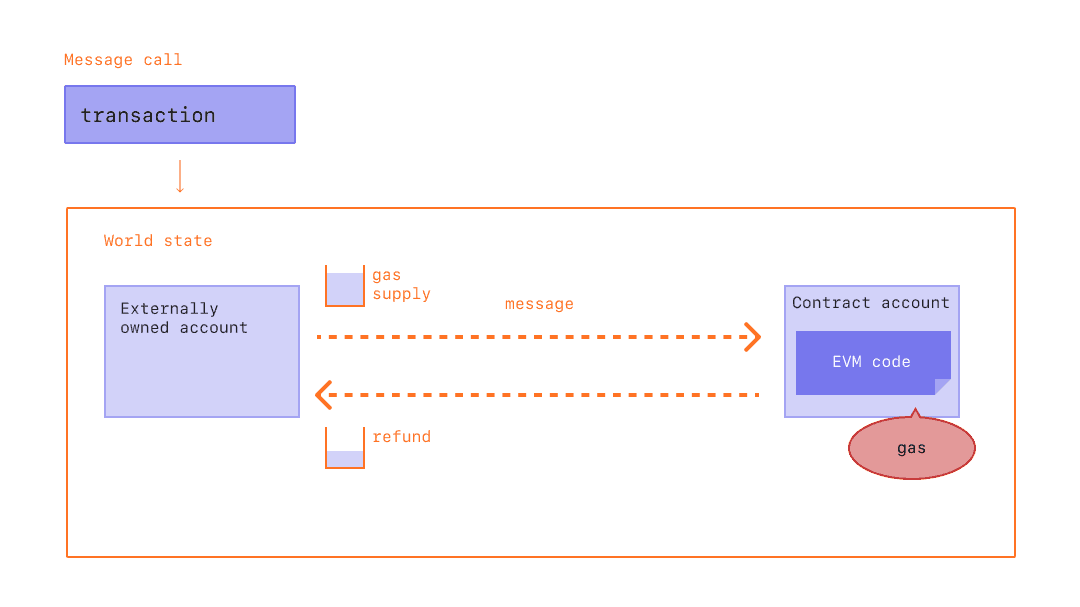
\includegraphics[width=1\textwidth]{img/capturas/gas.png}
    \caption{Diagrama que representa el reembolso del gas - Ethereum.org .}
    \label{fig:configApi}
\end{figure}


Por otro lado, cuando no hay gas suficiente, este gas se paga a los mineros por finalizar transacciones. Incluso si falla, los mineros deben validar y ejecutar la transacción.

\subsubsection{Redes}

Independientemente de la blockchain que usemos, si esta está basada en el protocolo Ethereum es probable que exista una red de pruebas\cite{testnets}. Por cada Mainnet ( blockchain principal ) hay una testnet ( red de pruebas ).

\bigskip

La red Mainnet es la principal, y es donde se despliegan los contratos en producción. El coste del despliegue suele ser alto, y una vez desplegado el contrato ya no se puede modificar. Por lo tanto es muy arriesgado desplegar en la mainnet sin tener una red donde poder realizar pruebas sobre el smart contract.

\bigskip

Las testnets son redes donde los desarolladores de smart contracts pueden desplegar sus contratos para probarlos. La criptomoneda de estas testnets no valen nada, y sirven únicamente para el propósito de probar el correcto funcionamiento del contrato a desplegar.

\bigskip

Los desarolladores pueden obtener criptomonedas desde cuentas "grifo"\cite{faucet} de forma gratuita para realizar las pruebas que crean oportunas sobre sus smart contracts. 

\bigskip

Un ejemplo de mainnet y testnet son las redes Polygon y Mumbai, que se usarán para este trabajo.

\subsubsection{Sobre Polygon}

Polygon es una red blockchain escalable que se enfoca en mejorar la eficiencia, la velocidad y la accesibilidad de Ethereum. Fue fundada en 2017 bajo el nombre de Matic Network y ha sido una de las soluciones de blockchain más exitosas en términos de escalabilidad y adopción en la comunidad Ethereum.

\bigskip

Polygon ofrece una capa adicional en la blockchain de Ethereum que permite la realización de transacciones rápidas y eficientes a través de un sistema de confirmación de bloques descentralizado y validación de transacciones a nivel de nodo. Además, Polygon es compatible con las aplicaciones y los contratos inteligentes existentes de Ethereum, lo que facilita la migración a la red.

\bigskip

Pros de Polygon:

\begin{itemize}
    \item Mejora en la escalabilidad: Polygon permite una mayor cantidad de transacciones por segundo y una confirmación de transacciones más rápida que Ethereum.
    \item Compatibilidad con Ethereum: Polygon es compatible con la mayoría de las aplicaciones y contratos inteligentes de Ethereum, lo que permite una migración sencilla a la red.
\end{itemize}

Contras de Polygon:

\begin{itemize}
    \item Menor seguridad: Debido a la estructura de la red, Polygon presenta un nivel de seguridad algo inferior al de Ethereum, aunque se están llevando a cabo esfuerzos para mejorarlo.
    \item Menor adopción: Polygon aún no ha alcanzado el mismo nivel de adopción que Ethereum, lo que puede limitar la cantidad de aplicaciones y contratos inteligentes disponibles en la red.
\end{itemize}

\subsubsection{Cuentas Externas y Cuentas de Contratos}

Una cuenta de Ethereum es una entidad con un saldo de ether (ETH) que puede enviar transacciones en Ethereum. Las cuentas pueden ser controladas por el usuario o implementadas como smart contracts.

\paragraph{Externas}

Estas cuentas representan una persona en la blockchain, su creación es gratuita y tienen claves publicas y privadas para poder acceder a ellas a través de una cartera, y firmar las transacciones.

\paragraph{Contratos}

Una cuenta de contrato en Ethereum es una dirección especial en la blockchain que apunta a una instancia de un contrato inteligente. Los contratos también tienen cuentas, ya que pueden albergar Ether y Tokens, y también ejecutar transacciones en la red, pero solo si alguien externo llama a una de sus funciones, ya que los contratos no pueden ejecutarse por si solos.

\subsubsection{Transacciones en Ethereum}

En Ethereum, una transacción representa una acción en la blockchain, como el envío de ETH o de un token basado en Ethereum de una cuenta a otra, la interacción con un contrato inteligente, o la modificación de los datos almacenados en la blockchain.

\bigskip

Cada transacción en Ethereum requiere una cantidad de gas para ser procesada y validada por los mineros de la red. Una vez que se realiza una transacción, se registra en la blockchain y se considera irrevocable.

\subsubsection{Solidity: Lenguaje Orientado a Smart Contracts}

En el caso de Ethereum, hay varias librerías para lenguajes como JS, Python o incluso C++ que nos permiten describir un smart contract y que compilan a bytecode que ejecuta la EVM ( Ethereum Virtual Machine ), aún así, se ha desarrollado un lenguaje específico para el desarrollo de smart contracts que compila a bytecode de EVM llamado Solidity.

\bigskip

Solidity\cite{soliditylang} es un lenguaje nos permite desarrollar Smart Contracts de forma cómoda, además Solidity posee sintaxis y definiciones que son similares a C++ y JS, aún así es importante no confundir Solidity como un lenguaje orientado a objetos, ya que este no entra en este paradigma.

\subsubsection{Comportamiento de un Smart Contract en Ethereum}

Un smart contract, al menos en Ethereum, se comporta muy similar a una API REST\cite{rest}. Cada contrato tiene un conjunto de funciones que se ejecutan sólo cuando se las llaman, estas pueden recibir, procesar, y devolver datos, además de alterar el estado de la blockchain, o incluso llamar a funciones de otros contratos.

\bigskip

Una vez desplegado un contrato, se genera una instancia de este en la blockchain en todos los nodos de la red, su código fuente no puede ser modificado y cada instancia es independiente.

\bigskip

Debido a que la EVM es una máquina de estados, al cambiar el valor de una variable de estado en nuestro contrato, lo que estamos haciendo en realidad es cambiar el estado de la blockchain.

\bigskip

Esto no significa que se esté sobreescribiendo dicho valor, en cambio se actualiza el valor más reciente para dicho espacio de almacenamiento en la blockchain.

\bigskip

En cualquier momento podemos ver los valores previos de estas variables a través del explorador de bloques, ya que cada cambio de estado es provocado por una transacción que debe ser minada, validada y finalmente archivada en un bloque.

\bigskip

Además, para cada contrato desplegado, se generan una cuenta de contrato, esto significa que el contrato en la blockchain tiene una dirección y una cartera para mantener Ether.

\bigskip

Una vez desplegado un contrato, para llamar a sus funciones deberemos saber la dirección del contrato, y la firma de la función ( identificador de función ).

\bigskip

A continuación se muestra ejemplo simple que de un smart contract hecho en Solidity que puede obtener, incrementar y decrementar un contador.

\bigskip

\lstinputlisting[language=Solidity, caption=Ejemplo de un Smart Contract en Solidity.]{codigo/ejemplos/contador.sol}


\subsubsection{Estructura de un smart contract con Solidity}

La estructura de un Smart Contract es bastante sencilla, los Smart Contracts en Solidity suelen tener principalmente un conjunto de variables globales ( variables de estado ), un constructor y funciones. 

\bigskip

A este programa se le puede añadir eventos, modificadores y librerías que se necesite importar, etc, pero al fin y al cabo cuando se interactua con un contrato, lo que se efecutará será una llamada a una función, o la lectura de un valor de una variable de estado.

\bigskip

\textbf{Variables - Almacenamiento}

\bigskip

Las variables de un contrato se guardan en 3 ubicaciones diferentes en la blockchain.

\begin{itemize}
    \item Storage: Persistente, se guarda en la blockchain.
    \item Memory: Variables locales / temporales, arrays.
    \item Calldata: Valores recibidos por parámetros de funciones, acceso externo.
\end{itemize}

Al igual que la RAM, Memory es un espacio temporal para almacenar datos durante la ejecución de un smart contract, pero se borra por completo una vez que la ejecución termina.

\bigskip

Storage, por otro lado, es persistente y los datos previamente almacenados en él están disponibles para cada ejecución del contrato. Sin embargo, su uso es costoso en términos de gas y se recomienda minimizar el número de accesos a las variables de estado. Las variables de estado solo se pueden declarar a nivel de contrato.

\bigskip

Calldata es similar a Memory y contiene los argumentos de la función, pero solo está disponible para los parámetros de llamadas a funciones externas.

\bigskip

En resumen, solo se debe especificar la zona de almacenamiento cuando se realizan transferencias de datos o al declarar variables dinámicas o secuenciales como arrays. Las variables en Memory solo se pueden declarar a nivel de función.

\bigskip

\lstinputlisting[language=Solidity, caption=Ejemplo de los diferentes espacios para alojar variables en Solidity.]{codigo/ejemplos/variables_almacenamiento.sol}

\newpage

\textbf{Variables - Tipos de datos}

\bigskip

En Solidity, existen diferentes tipos de variables que se pueden utilizar en un smart contract, como string, int, uint, arrays, etc. Además, es posible especificar el tamaño de la variable, por ejemplo: uint8, uint32, uint64, lo que permite reducir el costo de gas asociado con la asignación de memoria al interactuar con las variables.

\bigskip

Cuando no se especifica un tamaño, como en el caso de uint, se define con su tamaño máximo, es decir, uint = uint256.

\bigskip

Es importante tener en cuenta que el tamaño de la variable afecta la eficiencia de la asignación de memoria y, por lo tanto, también influye en el costo de gas asociado con la interacción con las variables.

\bigskip

\lstinputlisting[language=Solidity, caption=Ejemplo de los diferentes tipos de variables en Solidity.]{codigo/ejemplos/variables_tipos.sol}

\newpage

\bigskip

\textbf{Variables - Inmutables}

\bigskip

Las variables inmutables son aquellas que no pueden ser modificadas una vez se han establecido. Se pueden establecer valores para las variables inmutables dentro del constructor, pero no se pueden cambiar después. Las variables inmutables funcionan como constantes y se utilizan para almacenar valores que no deben ser modificados a lo largo del tiempo.

\bigskip

Al usar variables inmutables, se pueden asegurar que ciertos valores permanezcan constantes y sean confiables a lo largo de la ejecución del contrato. Esto es útil para establecer valores que se usan repetidamente en el código o para proporcionar una capa adicional de seguridad y prevenir errores involuntarios.

\bigskip

\lstinputlisting[language=Solidity, caption=Ejemplo de variables inmutables en Solidity.]{codigo/ejemplos/variables_inmutables.sol}

\bigskip

\textbf{Pragma y Licencias}

\bigskip

Las primeras 2 líneas de cada archivo .sol deben ser:

\begin{itemize}
    \item La licencia del código del archivo.
    \item La versión de compilador de solidity a usar.
\end{itemize}

Si no se especifica el compilador esperado en el smart contract, se generará un aviso. Esto es un recordatorio para el desarrollador para especificar la versión de compilador adecuada. Si se especifica un compilador y se compila con una versión diferente o incompatible, el proceso de compilación será abortado.

\bigskip

Esto es importante para garantizar la compatibilidad y evitar errores debido a cambios en la sintaxis o en las funciones disponibles en diferentes versiones del compilador de Solidity. Especificar la versión de compilador correcta garantiza que el contrato se compilará correctamente y funcionará como se esperaba.

\bigskip

\lstinputlisting[language=Solidity, caption=Ejemplo de pragma y licencia en los archivos .sol.]{codigo/ejemplos/pragma_y_licencia.sol}

En el ejemplo anterior se especifica que la licencia es GPL-3, y la versión del compilador debe ser superior o igual a 0.7.0 y inferior a la 0.9.0.


\bigskip

\textbf{Constructores}

\bigskip

El constructor de un smart contract es una función especial que se ejecuta automáticamente una sola vez, cuando se despliega el contrato en la blockchain. El constructor puede recibir argumentos o parámetros y utilizarlos para inicializar o configurar el estado inicial del contrato.

\bigskip

También es posible que un contrato herede de otro contrato y llame al constructor padre para inicializar algunos valores antes de continuar con su propia inicialización. Esto puede ser útil cuando se quiere reutilizar la lógica o los valores iniciales de otro contrato en un nuevo contrato.

\bigskip    

\lstinputlisting[language=Solidity, caption=Ejemplo de un constructor y herencias en Solidity.]{codigo/ejemplos/constructores.sol}

En la herencia de contratos no se hereda el estado actual del contrato padre, solo sus variables, funciones, valores iniciales, etc. No es posible heredar de un contrato ya desplegado, solo del código fuente. Además, también es posible crear interfaces en Solidity.

\newpage

\bigskip

\textbf{Visibilidad}

\bigskip

La visibilidad de una función o variable restringe su accesibilidad:

\begin{itemize}
    \item Public: Cualquiera puede llamar a la función, (usuario, otro contrato, función interna, contrato heredado ).

    \item External: Solo se puede llamar desde fuera del contrato actual, ( usuario, otro contrato ).

    \item Private: Solo contratos heredados o funciones internas pueden llamar a la función ( función  interna, contrato heredado ).

    \item Internal: Solo funciones internas del contrato actual pueden llamar a la función ( función interna ).
\end{itemize}

\bigskip 

\lstinputlisting[language=Solidity, caption=Ejemplo de visibilidades en funciones en Solidity.]{codigo/ejemplos/visibilidad_funciones.sol}

Cuando una variable es declarada como pública, el compilador genera un getter implícito, lo que significa que no es necesario crear un getter explícito para acceder a su valor. Sin embargo, aunque se utilice private o internal para restringir el acceso, esto no garantiza la ocultación del valor.

\bigskip 

La información almacenada en los contratos de Ethereum es pública y puede ser leída por cualquier persona en la blockchain mediante un block explorer. Es importante tener en cuenta que Ethereum es una blockchain pública y toda la información almacenada en los contratos es accesible para todos.

\bigskip 

\lstinputlisting[language=Solidity, caption=Ejemplo de visibilidades en variables en Solidity.]{codigo/ejemplos/visibilidad_variables.sol}

\bigskip

\textbf{Funciones}

\bigskip

Las funciones son el punto principal de interacción de un smart contract. A través de estas se proporciona la funcionalidad de la blockchain.


\bigskip

\textbf{Funciones - Mutabilidad}

\bigskip

La mutabilidad define si la función actual va a cambiar / acceder a alguna variable de estado, esto influye en el gasto de gas por el contrato, ya que si una función no cambia el estado de la blockchain tampoco habrá propagación, y por lo tanto se notifica a la EVM que no se necesita realizar una transacción para la ejecución de dicha función, esto hace que la llamada a dicha función sea gratuito. Las operaciones lógicas se ejecutarán sólo en un nodo.

\begin{itemize}
    \item View: Especifica que la función no va a modificar las variables de estado ( no se altera la blockchain ).

    \item Pure: Igual que la anterior pero que además especifica que no se va a leer de las variables de estado ( no se accede a la blockchain ).
\end{itemize}

\bigskip 

\lstinputlisting[language=Solidity, caption=Ejemplo de mutabilidades en Solidity.]{codigo/ejemplos/mutabilidad.sol}

\newpage

\bigskip

\textbf{Funciones - Returns }

\bigskip

Como se ha visto en el ejemplo anterior de mutabilidad, si una función devuelve un valor se debe especificar el tipo, si no devuelve nada no se requiere especificar nada.

\bigskip 

Se pueden declarar directamente las variable a devolver como un “contenedor”, la cual la función al acabar su ejecución devolverá automáticamente su valor. También se puede devolver múltiples variables.

\bigskip 

\lstinputlisting[language=Solidity, caption=Ejemplos de returns en Solidity.]{codigo/ejemplos/returns.sol}

\newpage

\bigskip

\textbf{Funciones - Payable }

\bigskip

Es posible habilitar que un contrato tenga un balance y pueda recibir transferencias de Ether, al igual que una cuenta normal.

\bigskip

Se puede acceder al balance actual del contrato utilizando la sintaxis \quotes{address(this).balance}. Además, es posible permitir que una función del contrato reciba Ether a través de la adición de la palabra "payable".

\bigskip

Esta misma palabra también se puede utilizar para transferir Ether desde el contrato a una cuenta.

\bigskip

La dirección de la cuenta que ha llamado a la función se puede acceder a través de \quotes{msg.sender}, y la cantidad de Ether enviada a través de \quotes{msg.value}.

\lstinputlisting[language=Solidity, caption=Ejemplo de un contrato usando Payable en Solidity.]{codigo/ejemplos/payable.sol}

\newpage

\bigskip

\textbf{Requires}

\bigskip

Durante la ejecución de una función se puede realizan comprobaciones llamadas "requires". En caso de fallar estas comprobaciones, se revierte la transacción con un mensaje de error personalizado, lo que significa que se deshacen todos los cambios realizados hasta ese momento.

\bigskip

El consumo de gas para la transacción solo ocurre hasta que se ejecuta la reversión. Esto se debe a que, aunque se reviertan todos los cambios, se requiere capacidad computacional para realizar estas operaciones.

\bigskip

\lstinputlisting[language=Solidity, caption=Ejemplo de sentencias require en Solidity.]{codigo/ejemplos/require.sol}

\newpage

\textbf{Modifiers}

\bigskip

Los modificadores son funciones auxiliares que se declaran con la sentencia “modifier”, y se adjuntan a otras funciones, de tal manera que la lógica de la función adjunta se ejecuta antes, durante o después de la auxiliar.

\bigskip

El carácter \quotes{\_} del modificador es reemplazado por la lógica de la función.

\bigskip

\lstinputlisting[language=Solidity, caption=Ejemplo del uso de modifiers en Solidity.]{codigo/ejemplos/modifiers_1.sol}

Los modifiers también soportan atributos.

\bigskip

\lstinputlisting[language=Solidity, caption=Ejemplo del uso de modifiers con parámetros en Solidity.]{codigo/ejemplos/modifiers_2.sol}

\newpage

\bigskip

\textbf{Funciones por defecto.}

\bigskip

En Solidity hay 2 funciones que nos permiten definir el comportamiento del contrato ante ciertas circunstancias:

\begin{itemize}
    \item receive() external payable: Se ejecuta si el contrato solo recibe ether mediante una transferencia normal, sin que se haya llamado a ninguna función payable ( recordemos que un contrato al fin y al cabo es una cuenta, y puede recibir transferencias ordinarias ).

    \item fallback() external payable: Si la función que se ha llamado no está definida en el contrato.
\end{itemize}

\bigskip

Por defecto, estas funciones no están definidas, sin embargo, si se requiere implementar alguna lógica específica en caso de que se produzca alguna de las situaciones mencionadas anteriormente, basta con definir la función con el nombre y los parámetros especificados previamente.

\bigskip

\lstinputlisting[language=Solidity, caption=Ejemplo del uso de funciones por defecto en Solidity.]{codigo/ejemplos/defaults.sol}

\newpage

\bigskip

\textbf{Transacciones}

\bigskip

En Solidity tenemos 3 maneras de enviar ether desde nuestro contrato a un usuario u otro contrato.

\begin{itemize}
    \item Send: devuelve false si falla, gas NO ajustable.
    \item Transfer: revierte si falla, gas NO ajustable.
    \item Call\{value\}(\quotes{}): devuelve false si falla, gas ajustable.
\end{itemize}

\bigskip

\lstinputlisting[language=Solidity, caption=Ejemplo de transferencia de Ether  en Solidity.]{codigo/ejemplos/send.sol}

\newpage

\bigskip

\textbf{Llamadas Externas}

\bigskip

Como ya se ha mencionado, un contrato puede llamar a otro contrato ( de una función a otra ).

Para hacer esto tenemos 2 maneras:

\begin{itemize}
    \item Usando el código del contrato, o una Interfaz.

    \lstinputlisting[language=Solidity, caption=Ejemplo de llamada externa usando el código del contrato destinatario en Solidity.]{codigo/ejemplos/external_1.sol}

\newpage
    
    \item Especificando el método en la llamada, al especificar el método, “abi.encodeWithSignature” genera el identificador de la función para el contrato a llamar.

    \lstinputlisting[language=Solidity, caption=Ejemplo de llamada externa usando el identificador de la función destinataria en Solidity.]{codigo/ejemplos/external_2.sol}
    
\end{itemize}

\newpage

\bigskip

\textbf{Eventos}

\bigskip

Los eventos sirven para registrar un historial de acciones que suceden en el contrato para poder acceder a ellos posteriormente de forma cómoda. Se suele usar para indexar datos en la blockchain y poder leerlos sin tener que buscar bloque a bloque usando un explorador de bloques\cite{etherscan}.

\bigskip

\lstinputlisting[language=Solidity, caption=Ejemplo del uso y definición de eventos en Solidity.]{codigo/ejemplos/events.sol}

\bigskip

\textbf{Optimización del gas}

\bigskip

Debido a que en la EVM, las variables de Storage se guardan en ranura de 32 bytes, al declarar las variables de estado se pueden empaquetar en ranuras de 32 bytes para optimizar el acceso a dicho pack, ya que cuando se lee o guarda una variable de estado, se lee la ranura entera de 32 bytes, y se accede a cada posicion individualmente.

\bigskip

Empaquetar tus variables significa que empaquetas o juntas variables de menor tamaño para que en conjunto formen 32 bytes.

\bigskip

Por ejemplo, puede empaquetar 32 uint8 en una ranura de almacenamiento, pero para que eso suceda, es importante que se declaren consecutivamente porque el orden de declaración de las variables importa en Solidity.

\newpage

\bigskip

\textbf{Librerías}

\bigskip

Las librerias en Solidity son bloques de código reutilizables que se pueden integrar en diferentes contratos inteligentes. Las bibliotecas son útiles porque permiten evitar la duplicación de código y mejoran la legibilidad y la organización del código.

\bigskip

SafeMath es una biblioteca popular en Solidity que proporciona funciones matemáticas seguras para evitar errores comunes, como desbordamientos y subdesbordamientos. 

\bigskip

Aquí hay un ejemplo sencillo de un contrato inteligente que utiliza la biblioteca SafeMath:

\bigskip

\lstinputlisting[language=Solidity, caption=Ejemplo del uso de la libreria SafeMath en Solidity.]{codigo/ejemplos/librerias.sol}

En este ejemplo, importamos la biblioteca SafeMath desde GitHub y la hacemos disponible en el contrato inteligente utilizando la sentencia using SafeMath for uint256;. Luego, utilizamos las funciones add y sub de SafeMath para realizar operaciones matemáticas seguras en las funciones deposit y withdraw.

\subsubsection{Estandards}

Los estándares son convenios técnicos utilizados para definir la funcionalidad de los tokens en la cadena de bloques Ethereum. Estos estándares establecen un conjunto de reglas para la creación, emisión y transferencia de tokens en la red Ethereum. Los estándares más populares incluyen \textcolor{blue}{\href{https://eips.ethereum.org/EIPS/eip-20}{\textbf{ERC-20}}}\footnote{\url{https://eips.ethereum.org/EIPS/eip-20}}, \textcolor{blue}{\href{https://eips.ethereum.org/EIPS/eip-721}{\textbf{ERC-721}}}\footnote{\url{https://eips.ethereum.org/EIPS/eip-721}} y \textcolor{blue}{\href{https://eips.ethereum.org/EIPS/eip-1155}{\textbf{ERC-1155}}}\footnote{\url{https://eips.ethereum.org/EIPS/eip-1155}}.

\subsubsection{OpenZeppelin}

\textcolor{blue}{\href{https://www.openzeppelin.com/}{\textbf{OpenZeppelin}}}\footnote{\url{https://www.openzeppelin.com/}} es una organización que provee estandars y una biblioteca de contratos inteligentes de código abierto y seguro para Ethereum, que proporciona herramientas y soluciones comunes para desarrolladores de contratos inteligentes. OpenZeppelin incluye una amplia gama de contratos inteligentes preconstruidos y estandares de tokens, que se pueden utilizar como una base sólida para la construcción de nuevos contratos inteligentes.

\paragraph{ERC-20 - Tokens}

Un token ERC-20 es un tipo de token en la plataforma Ethereum que se adhiere al estándar ERC-20. ERC-20 es un estándar técnico que describe cómo se deben crear, emitir y transferir tokens en la red Ethereum.

\bigskip

El estándar ERC-20 incluye una serie de funciones y eventos que deben implementarse en un contrato inteligente para que sea considerado un token ERC-20. Algunos de los requisitos incluyen la implementación de funciones para obtener la información sobre el token, como el nombre, la simbología, el número total de tokens emitidos, etc.

\subsubsection{ABIs}

Los compiladores de Solidity también generan información adicional, como la ABI (Interfaz de Programación de Aplicaciones), que se utiliza para interactuar con el contrato inteligente a través de una aplicación o una interfaz.

\subsubsection{Dapps}

Las DAPPS (aplicaciones descentralizadas) son aplicaciones que funcionan con contratos inteligentes para llevar a cabo sus tareas.

\bigskip

Estas se construyen utilizando tecnologías blockchain como Ethereum, que les permiten tener una base de datos distribuida y un sistema de consenso descentralizado que asegura la integridad y seguridad de los datos.

\bigskip

Esto significa que las DAPPS son resistentes a la manipulación y la censura, y se les considera más seguras y privadas que las aplicaciones tradicionales que dependen de

\subsubsection{Sistemas}

En Ethereum, se pueden desarollar diferentes tipos de sistemas usando, contratos inteligentes, estandares, librerias, etc ...

\bigskip

Los más comunes en la red suelen ser los siguientes:

\paragraph{ICO}

Una ICO (Oferta Inicial de Monedas) es un tipo de financiación de proyectos en el mundo de las criptomonedas y la tecnología blockchain. Se trata de una oferta de venta de tokens digitales a inversores en una etapa temprana del proyecto, con el objetivo de recaudar fondos para su desarrollo.

\bigskip

Los inversores que participan en una ICO compran tokens con una criptomoneda establecida, como Bitcoin o Ethereum, o con dinero fiat. Luego, pueden mantener esos tokens o venderlos en un intercambio de criptomonedas cuando su valor aumente.

\bigskip

Las ICO se han utilizado para financiar una amplia variedad de proyectos en el mundo de las criptomonedas, desde nuevas criptomonedas hasta plataformas descentralizadas y aplicaciones descentralizadas (DAPPs).

\paragraph{DAO}

Una DAO (Organización Descentralizada Autónoma) es un tipo de organización que se basa en la tecnología blockchain y utiliza contratos inteligentes para tomar decisiones y ejecutar acciones.

\bigskip

Estos sistemas compuestos por smart contracts son descentralizadas y autónomas, lo que significa que no tienen una estructura jerárquica centralizada y que sus decisiones y acciones son tomadas y ejecutadas automáticamente por sus contratos inteligentes, sin la necesidad de una intermediación humana.

\bigskip

Los participantes tienen derecho a voto en proporción a la cantidad de tokens que poseen. Estos tokens se adquieren mediante una inversión en la DAO y representan una participación en la organización.

\paragraph{DEX}

Una DEX (Bolsa Descentralizada) es un tipo de plataforma de intercambio de criptomonedas que utiliza la tecnología blockchain y contratos inteligentes para permitir la negociación peer-to-peer de activos digitales.

\bigskip

A diferencia de las bolsas centralizadas, que tienen una entidad central que controla los activos y las operaciones de los usuarios, las DEX son descentralizadas y no dependen de intermediarios centralizados. Esto significa que los usuarios tienen un mayor control sobre sus activos y sus operaciones, y que no hay una sola entidad que tenga acceso a los fondos de los usuarios.

\bigskip

Las DEX funcionan mediante la utilización de contratos inteligentes en una blockchain, que se encargan de gestionar las órdenes de compra y venta y de ejecutar automáticamente las transacciones.

\bigskip

Estos contratos inteligentes también garantizan la seguridad y la transparencia de las operaciones, ya que se ejecutan en una blockchain descentralizada.

\newpage

\subsection{IPFS}

\textcolor{blue}{\href{https://ipfs.tech/}{\textbf{IPFS}}}\footnote{\url{https://ipfs.tech/}} es el acrónimo de Inter Planetary File System y es un sistema de archivos distribuido que utiliza la tecnología de blockchain. A diferencia de la tecnología de archivos convencional que utiliza servidores centralizados, IPFS utiliza una red descentralizada de nodos para almacenar y compartir archivos.

\bigskip

Esto significa que, en lugar de alojar archivos en un servidor centralizado, los archivos son fragmentados en pequeñas piezas y almacenados en múltiples nodos en la red IPFS.

\bigskip

Cuando alguien quiere acceder a un archivo, se descarga de los nodos que lo tienen, en lugar de un servidor central y cada archivo en la red se identifica mediante un hash único generado por una función de hash criptográfica, y a los cuales se puede acceder usando una dirección URL.

\bigskip

IPFS es una tecnología de blockchain porque utiliza la criptografía para garantizar la integridad y la autenticidad de los archivos en la red. Además, los archivos se identifican mediante una dirección única y permanente generada por un hash criptográfico, lo que significa que los archivos no pueden ser modificados o alterados sin ser detectados.

\bigskip

\begin{figure}[H]
        \centering
        \includegraphics[width=1\textwidth]{img/capturas/ipfs.png}
        \caption{Panel de control del Cliente IPFS.}
        \label{fig:configApi}
\end{figure}

En este trabajo se usa IPFS como un medio donde almacenar imágenes y videos asociados a las propuestas de proyectos.

\newpage

\subsection{EtherJS}

\textcolor{blue}{\href{https://docs.ethers.org/v5/}{\textbf{Ethers}}}\footnote{\url{https://docs.ethers.org/v5/}} es una libreria de JavaScript que permite la conexión de una aplicación desarollada en JS a cualquier blockchain que esté usando el protocolo Ethereum.

\bigskip

\lstinputlisting[language=JavaScript, caption=Ejemplo de conexión a una cartera Metamask usando Ethers.]{codigo/ethers/ejemplo.js}

\bigskip

La librería provee de un conector dada la dirección de un nodo de la red, y de métodos para interactuar con los smart contracts mediante el uso de una ABI y un firmante mediante ( cuenta de la blockchain ) una cartera.

\subsection{Svelte}

\textcolor{blue}{\href{https://svelte.dev/}{\textbf{Svelte}}}\footnote{\url{https://svelte.dev/}} es un framework de desarrollo web basado en JavaScript que facilita la creación de interfaces de usuario. A diferencia de otros frameworks populares como React o Vue, Svelte se enfoca en compilar los componentes durante el proceso de construcción en lugar de ejecutarlos en tiempo de ejecución en el navegador del cliente, esto resulta en un rendimiento superior y una menor carga en los recursos del navegador.

\bigskip

Los componentes de Svelte están escritos en un archivo \quotes{.svelte} que combina el HTML, CSS y JavaScript necesarios para el componente. Esto permite una mejor separación de responsabilidades y una mayor legibilidad del código.

\bigskip

\lstinputlisting[language=JavaScript, caption=Hello World en Svelte.]{codigo/svelte/ejemplo.js}

\bigskip

Para este trabajo se ha seleccionado este framework por su realmente reactividad, y sus patrón basado en componente para desarollar las vistas del front-end.

\subsection{HardHat}

\textcolor{blue}{\href{https://hardhat.org/}{\textbf{Hardhat}}}\footnote{\url{https://hardhat.org/}} es un entorno de desarrollo de smart contracts desarrollado en JavaScript, este nos permite compilar código en Solidity, desplegar nodos con cuentas de prueba localmente, para testear nuestros contratos y finalmente desplegarlos.

\bigskip

\begin{figure}[H]
        \centering
        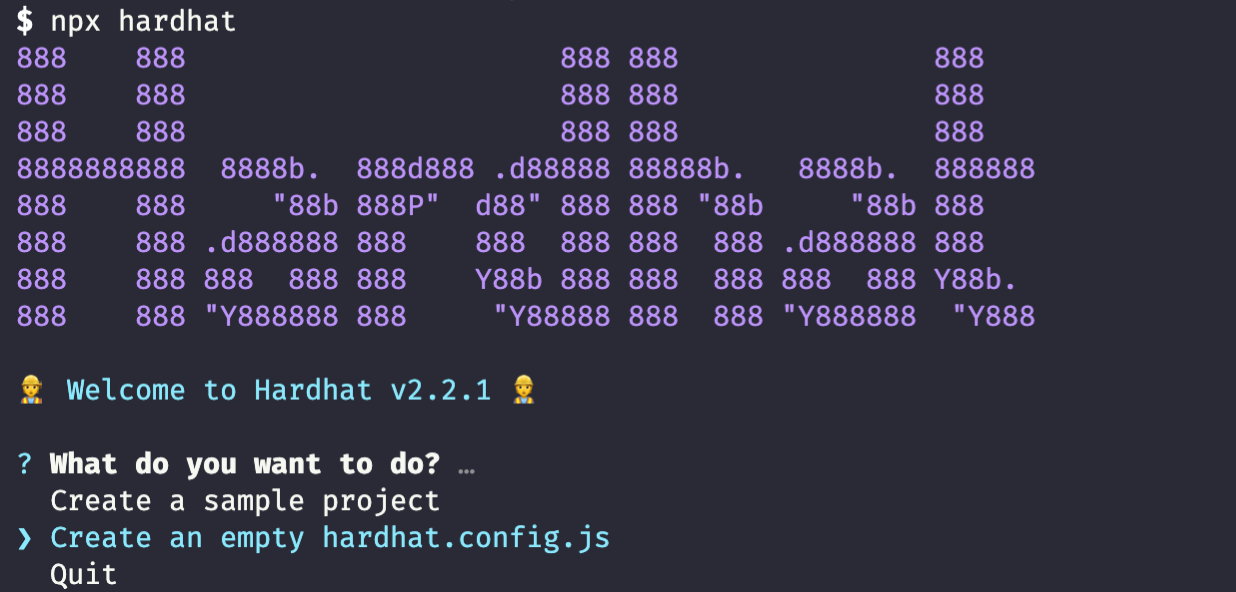
\includegraphics[width=1\textwidth]{img/capturas/hardhat.png}
        \caption{Console del cliente de HardHat.}
        \label{fig:configApi}
\end{figure}

\bigskip

Es altamente configurable además de soportar tests unitarios para nuestros contratos. Se pueden programar \quotes{tasks} para automatizar ciertos procesos como la verificación de contratos en los block explorers como Etherscan.

\newpage

\subsection{ThirdWeb}

\textcolor{blue}{\href{https://thirdweb.com/}{\textbf{ThirdWeb}}}\footnote{\url{https://thirdweb.com/}} es un framework de desarollo de DApps, con un amplio abanico de librerias que permiten facilitar la integración de funcionalidades basadas en blockchain en aplicaciones desarolladas en JavaScript. 

\bigskip

De este framework se restalta la libreria \quotes{thirdweb-dev/storage} que provee de la funcionalidad de conectarse mediante JavaScript a la blockchain IPFS, subir documentos, y obtener su hash unico. 

\bigskip

\lstinputlisting[language=JavaScript, caption=Ejemplo de la conexión y subida de un archivo a IPFS.]{codigo/thirdweb/ejemplo.js}

\subsection{Bootstrap}

\textcolor{blue}{\href{https://getbootstrap.com/}{\textbf{Bootstrap}}}\footnote{\url{https://getbootstrap.com/}} es un framework de diseño web de código abierto que proporciona una colección de herramientas, componentes y estilos para ayudar a los desarrolladores a crear sitios y interfaces responsive\footnote{El término se refiere a la capacidad de un sitio web para adaptarse a diferentes tamaños de pantalla, desde pantallas pequeñas de dispositivos móviles hasta pantallas grandes de escritorio.}.

\bigskip

\begin{figure}[H]
        \centering
        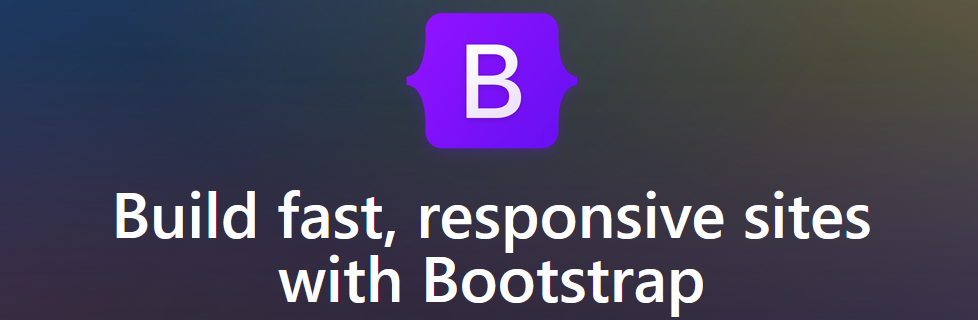
\includegraphics[width=0.7\textwidth]{img/capturas/bootstrap.png}
        \caption{Logotipo y slogan de Bootstrap.}
        \label{fig:configApi}
\end{figure}

\bigskip

Bootstrap está basado en HTML, CSS y JavaScript y permite a los desarrolladores crear diseños personalizados, así como utilizar estilos predefinidos, también incluye una cuadrícula de diseño flexible que permite a los desarrolladores crear diseños complejos y alinear fácilmente.

\newpage

\subsection{MetaMask}

\textcolor{blue}{\href{https://metamask.io/}{\textbf{MetaMask}}}\footnote{\url{https://metamask.io/}} es una cartera que nos permite gestionar nuestra cuenta de Ethereum, pero que además existe en formato de extensión de navegador, esto hace más seguro y fácil desarrollar e interactuar con interfaces web que conectan con un contrato.

\begin{figure}[H]
        \centering
        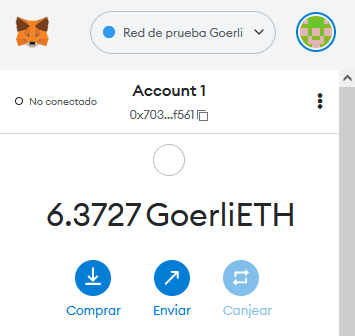
\includegraphics[width=0.5\textwidth]{img/capturas/metamask.png}
        \caption{Captura de la cartera de MetaMask.}
        \label{fig:configApi}
\end{figure}

\bigskip

MetaMask provee al navegador de una variable en JS \quotes{window.ethereum}, la cual después es usada por librerías como Ethers para interactuar con la blockchain desde las DApps.

\bigskip

Esta variable, posee entre otros, un objeto que representa al firmante ( la cuenta ethereum del usuario ) y la conexión al nodo incluyendo la dirección JSONRCP, estos datos son fundamentales para poder interactuar con los smart contracts.

\newpage

\subsection{Docker}

\textcolor{blue}{\href{https://www.docker.com/}{\textbf{Docker}}}\footnote{\url{https://www.docker.com/}} es una plataforma de software que permite a los desarrolladores crear, ejecutar y distribuir aplicaciones en contenedores. Los contenedores son unidades de software portátiles y livianas que contienen todas las dependencias y configuraciones necesarias para que una aplicación se ejecute de manera eficiente y confiable, independientemente del entorno en el que se esté ejecutando.

\begin{figure}[H]
        \centering
        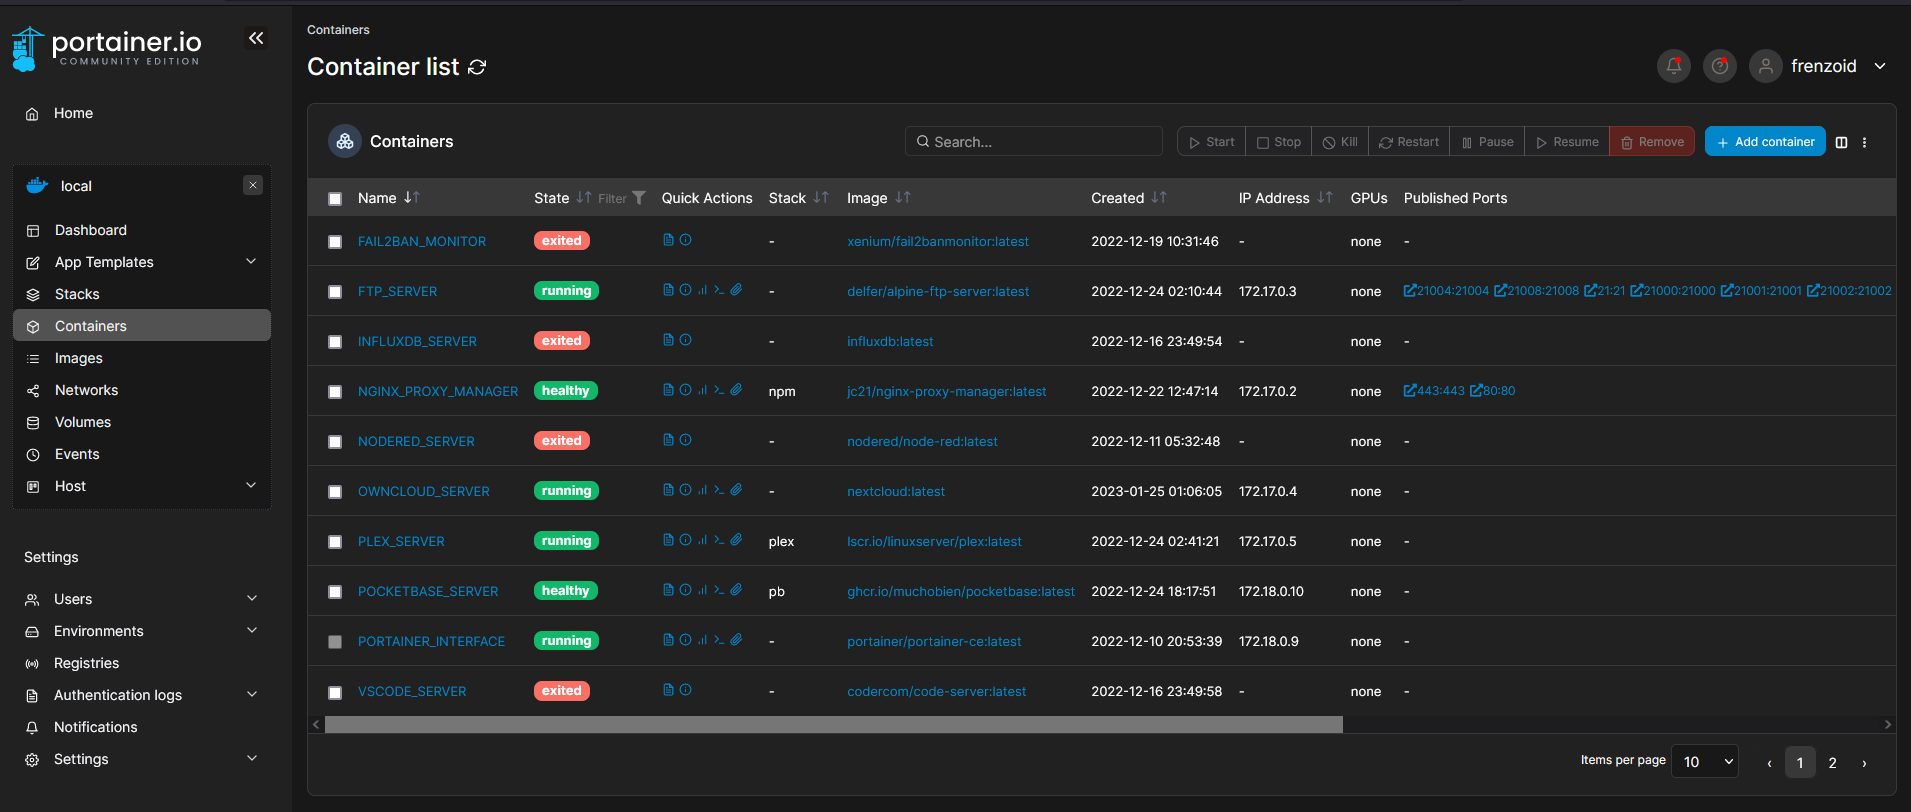
\includegraphics[width=1\textwidth]{img/capturas/portainer.png}
        \caption{Captura del panel de control de Portainer.}
        \label{fig:configApi}
\end{figure}

\bigskip

En este trabajo, se usará Docker para desplegar el front-end en un servidor, una vez haya finalizado el proyecto. También usaremos \textcolor{blue}{\href{https://www.portainer.io/}{\textbf{Portainer}}}\footnote{\url{https://www.portainer.io/}}, un contenedor que nos provee de una aplicación web para gestionar los contenedores de nuestro servidor.